\documentclass[12pt,letterpaper]{article}
%\documentstyle[11pt]{article}
\usepackage[utf8]{inputenc}
\usepackage{amsmath}
\usepackage{xfrac}
\usepackage{amsfonts}
\usepackage{amssymb}
\usepackage[version = 3]{mhchem}
\usepackage{chemstyle}
%%For Table perhaps%%
%\usepackage{graphics}
\usepackage{graphicx}
\usepackage{epstopdf}
\usepackage{tabularx,ragged2e,booktabs,caption}
%\newcolumntype{C}[1]{>{\Centering}m{#1}}
%\renewcommand\tabularxcolumn[1]{C{#1}}
\usepackage[left=1.5cm,right=1.5cm,top=0.5cm,bottom=2cm]{geometry}
\usepackage{subcaption} 
\usepackage{caption}
\usepackage[colorlinks]{hyperref}
\usepackage[svgnames]{xcolor}
\hypersetup{citecolor=DeepPink4}
\hypersetup{linkcolor=DarkRed}
\hypersetup{urlcolor=DarkBlue}
\usepackage{cleveref}

\begin{document}
\setlength{\parindent}{0cm} 


\frenchspacing


\title {\Large{\textbf{Quiz 5---BOD}}\\ \large{CENG 340--Introduction to Environmental Engineering\\
Instructor: Deborah Sills\\ \textbf{8 November, 2013}}}
\author {}
\date {}
\maketitle

\vspace{-0.4 in}
\textbf{\large{Name:}}\\



The figure below shows a plot of BOD remaining versus time taken from a wastewater treatment plant.  The data came from a BOD test which was run at 20 $^0$C with a total sample size of 200 mL.  In other words, the test was run in a 200 mL BOD bottle.

\vspace{0.1in}

\begin{figure}
\centering
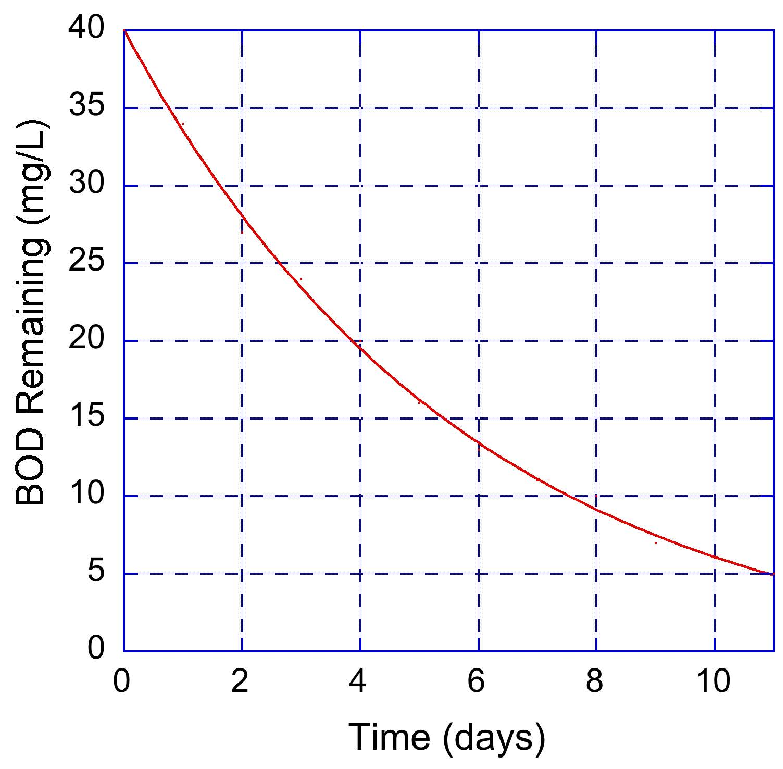
\includegraphics[width=0.4\textwidth]{quiz_bod_take2}
\end{figure}

\vspace{-0.1in}

\begin{enumerate}
\item  What is the ultimate BOD (L$_0$)?
\vspace{0.5in} [2.5 pt]

\item What is L$_5$?
\vspace{0.5in} [2.5 pt]

\item How much oxygen (in mg/L) was consumed during the first 5 days of the BOD test?
\vspace{0.5in} [2.5 pt]
\item How much oxygen (in mg) was consumed during the first 5 days of the BOD test? [2.5 pt]

\end{enumerate}






\end{document}